% =====================================================================
% Přednáška 3 (17. 10. 2022): formfaktor, účinné průřezy, vlastnosti jader,
% kapkový model, jednočásticové modely (deuteron), slupkový model,
% kolektivní stavy
% =====================================================================
\section{Formfaktor, vlastnosti jader a modely jádra}

\strana{P03-1}
\subsection{Rozptyl na rozloženém náboji: formfaktor}

Na minulé přednášce jsme odvodili diferenciální účinný průřez rozptylu nabité
částice na \emph{bodovém} rozptylovém centru. V kvantové teorii rozptylu je
popsán \kw{rozptylovou amplitudou} \(f\), která závisí jen na
\kw{přenesené hybnosti} \(\vec q\) (v jednotkách \(\hbar=1\) je
\(\vec q = \vec k - \vec k'\) rozdíl vlnových vektorů dopadající a rozptýlené
vlny, tj.\ \(\hbar\vec q\) je hybnost předaná terči):
\[
  \frac{\dd\sigma}{\dd\Omega} = \abs{f(\vec q)}^2 .
\]
Pro Coulombovo pole bodového náboje dává tento vzorec Rutherfordův průřez
\(\propto 1/\sin^4(\theta/2)\). Skutečné terče -- jádra, ale i nukleony -- však
bodové nejsou: jejich náboj je rozprostřen v nějakém objemu. Chceme proto
zjistit, jak se rozložení náboje projeví v měřeném průřezu, a naopak, jak
z měřeného průřezu \emph{rozložení náboje zrekonstruovat}. Přesně tímto
způsobem se historicky měřil poloměr jader (R.~Hofstadter, rozptyl
vysokoenergetických elektronů, viz Davídkovy slajdy \uv{Rozměr jádra}).

Úvaha je jednoduchá. Kdyby bodové rozptylové centrum neleželo v počátku, ale
v bodě \(\vec x_i\), amplituda by se změnila jen o fázový faktor (dopadající
vlna \(e^{i\vec k\cdot\vec x}\) a rozptýlená vlna \(e^{i\vec k'\cdot\vec x}\)
mají v bodě \(\vec x_i\) relativní fázi \(e^{i(\vec k-\vec k')\cdot\vec x_i}\);
znaménko v exponentu je věc konvence):
\[
  f(\vec q) \;\longrightarrow\; f(\vec q) \;\longrightarrow\; f(\vec q)\,e^{-i\vec q\cdot\vec x_i}.
\]
Je-li náboj rozložen spojitě s normovanou hustotou \(\rho(\vec x)\)
(\(\int\rho\,\dd^3x = 1\)), sečteme (přesněji zintegrujeme) příspěvky všech
elementů náboje -- amplitudy se sčítají \emph{koherentně}, tedy včetně fází:
\[
  \vzorec{\frac{\dd\sigma}{\dd\Omega} = \abs{f(\vec q)\,F(\vec q)}^2},
  \qquad
  \vzorec{F(\vec q) = \int \rho(\vec x)\,e^{-i\vec q\cdot\vec x}\,\dd^3x } .
\]

\begin{definice}[Formfaktor]
\kw{Formfaktor} \(F(\vec q)\) je Fourierova transformace (normované) hustoty
rozložení náboje terče. Účinný průřez na rozloženém náboji je průřez na
bodovém náboji vynásobený \(\abs{F(\vec q)}^2\).
\end{definice}

Smysl je tedy tento: změříme \(\dd\sigma/\dd\Omega\), vydělíme známým
průřezem na bodovém náboji (Rutherford, resp.\ Mott pro relativistické
elektrony), dostaneme \(\abs{F(q)}^2\) a zpětnou Fourierovou transformací
odhadneme \(\rho(\vec x)\).

\subsubsection*{1. Sféricky symetrické rozložení \(\rho(\vec x)=\rho(r)\)}

Pro jádra je přirozené předpokládat sférickou symetrii. Nejprve limitní
případ: pro \(q\to 0\) je \(e^{-i\vec q\cdot\vec x}\to 1\) a díky normování
\[
  q\to 0 \;\Rightarrow\; F(\vec q) = 1 .
\]
Fyzikálně: při malé přenesené hybnosti má sonda velkou vlnovou délku
\(\sim 1/q\) a \uv{nevidí} vnitřní strukturu terče -- ten se jeví jako
bodový.

Pro sféricky symetrickou hustotu lze úhlovou integraci provést (osu \(z\)
zvolíme podél \(\vec q\)): \(\int e^{-iqr\cos\vartheta}\dd\Omega
= 4\pi\,\frac{\sin(qr)}{qr}\), takže
\(F(q) = \frac{4\pi}{q}\int_0^\infty \rho(r)\,r\sin(qr)\,\dd r\). Formfaktor
tedy závisí jen na velikosti \(q=\abs{\vec q}\). Pro malá \(q\) rozvineme sinus
do Taylorovy řady \(\sin x = x - x^3/6 + \dots\):
\begin{align*}
  F(q) &\doteq \frac{4\pi}{q}\int_0^\infty \rho(r)\,r\left(qr - \frac{(qr)^3}{6} + \dots\right)\dd r = \\
  &= 4\pi\int_0^\infty \rho(r)\,r^2\,\dd r - \frac{4\pi q^2}{6}\int_0^\infty \rho(r)\,r^4\,\dd r
   = 1 - \frac{q^2}{6}\int_0^\infty 4\pi\rho(r)\,r^4\,\dd r = \\
  &= \vzorec{1 - \frac{q^2}{6}\,\langle r^2\rangle} .
\end{align*}
První integrál je právě normování (\(4\pi r^2\dd r\) je objem slupky), druhý
je střední hodnota \(r^2\) vážená hustotou náboje, tedy \kw{střední kvadratický
poloměr} \(\langle r^2\rangle\).

\begin{veta}[Formfaktor při malých \(q\)]
Sklon formfaktoru v okolí \(q=0\) určuje střední kvadratický poloměr terče
nezávisle na detailním tvaru \(\rho(r)\):
\(F(q)\approx 1-\tfrac{1}{6}q^2\langle r^2\rangle\).
Odtud se měří \uv{velikost} jader i protonu.
\end{veta}

Pro větší \(q\) už formfaktor závisí na tvaru rozložení. Dva modelové
příklady:

\textbf{1a: formfaktor vodivé nabité koule.} Na vodivé kouli sedí veškerý
náboj na povrchu, tj.\ v tenké slupce o poloměru \(R\):
\[
  \rho = \frac{1}{4\pi R^2}\,\delta(r-R)
  \qquad\Rightarrow\qquad
  F(q) = \frac{\sin(qR)}{qR} .
\]
(Dosazení do \(F(q)=\frac{4\pi}{q}\int\rho\,r\sin(qr)\,\dd r\) je
okamžité.)

\textbf{1b: formfaktor homogenně nabité koule.} Náboj rovnoměrně rozložený
v objemu koule:
\[
  \rho = \frac{1}{\frac{4\pi}{3}R^3}\quad\text{pro } r<R
  \qquad\Rightarrow\qquad
  F(q) = \frac{3}{q^3R^3}\Big[\sin(qR) - qR\cos(qR)\Big] .
\]
(Integrál \(\int_0^R r\sin(qr)\,\dd r = [\sin(qR)-qR\cos(qR)]/q^2\) se spočte
per partes.) Rozvojem pro malé \(qR\) se snadno ověří, že
\(F\approx 1 - q^2R^2/10\), tj.\ \(\langle r^2\rangle = \frac35R^2\), což
souhlasí s obecným výsledkem výše.

\begin{vysvetleni}[Jak vypadají formfaktory -- difrakční minima]
Oba formfaktory oscilují a mají nulové body, podobně jako difrakční obrazec
světla na kruhovém otvoru. Pro slupku jsou nuly v \(qR=n\pi\), pro homogenní
kouli v řešeních \(\tan(qR)=qR\) (první v \(qR\approx4{,}49\)). Poloha
prvního minima v naměřeném \(\abs{F(q)}^2\) proto přímo udává poloměr
\(R\). Reálná jádra mají \uv{rozmazaný} okraj (Fermiho rozdělení), takže
minima nejsou úplně nulová, ale jsou dobře viditelná -- právě tak Hofstadter
v 50.~letech změřil \(R\approx1{,}2\,A^{1/3}\)\,fm.
\begin{center}
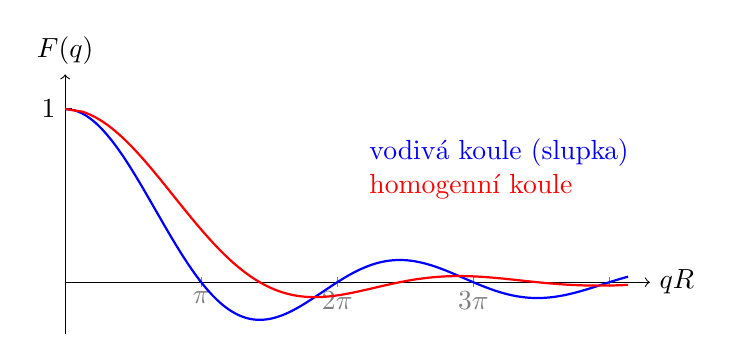
\begin{tikzpicture}[x=0.55cm,y=2.2cm]
  \draw[->] (0,0) -- (13.5,0) node[right] {\(qR\)};
  \draw[->] (0,-0.3) -- (0,1.2) node[above] {\(F(q)\)};
  \draw (0,1) node[left] {\(1\)} -- (0.15,1);
  \foreach \x in {3.1416,6.2832,9.4248,12.566}
    \draw[gray] (\x,0.03) -- (\x,-0.03);
  \node[below,gray] at (3.1416,0) {\(\pi\)};
  \node[below,gray] at (6.2832,0) {\(2\pi\)};
  \node[below,gray] at (9.4248,0) {\(3\pi\)};
  \draw[thick,blue] (0,1) -- plot[domain=0.2:13,samples=150,smooth] (\x,{sin(\x r)/\x});
  \draw[thick,red] (0,1) -- plot[domain=0.4:13,samples=150,smooth] (\x,{3*(sin(\x r)-\x*cos(\x r))/(\x*\x*\x)});
  \node[blue,right] at (6.8,0.75) {vodivá koule (slupka)};
  \node[red,right] at (6.8,0.55) {homogenní koule};
\end{tikzpicture}
\end{center}
\end{vysvetleni}

\strana{P03-2}
\subsection{Příklad účinných průřezů}

Abychom získali představu o číslech, uveďme účinné průřezy pro záchyt
\emph{tepelných} (pomalých) neutronů na několika jádrech
(\(1\,\mathrm{b} = 10^{-28}\,\mathrm{m}^2 = 100\,\mathrm{fm}^2\)):
\[
\begin{array}{lcl}
  n + {}^{2}\mathrm{H}   &:& \sigma \sim 5\cdot10^{-4}\,\mathrm{b} \\
  n + {}^{16}\mathrm{O}  &:& \sigma \sim 2\cdot10^{-4}\,\mathrm{b} \\
  n + {}^{113}\mathrm{Cd} &:& \sigma \sim 2\cdot10^{4}\,\mathrm{b} \\
  n + {}^{135}\mathrm{Xe} &:& \sigma \sim 3\cdot10^{6}\,\mathrm{b}
\end{array}
\]
Rozptyl hodnot je obrovský -- deset řádů! Geometrický průřez jádra
\(\pi R^2\) přitom činí řádově desetiny až jednotky barnu (pro těžké jádro
s \(R\approx 7\,\mathrm{fm}\) je \(\pi R^2\approx 1{,}5\,\mathrm{b}\)). Jak
může být průřez o mnoho řádů \emph{větší}, než je samotné jádro? Odpověď
dává vlnová délka tepelného neutronu.

\begin{priklad}[Vlnová délka tepelného neutronu]
Tepelný neutron je v rovnováze s prostředím o teplotě \(T = 300\,\mathrm{K}\),
tj.\ má kinetickou energii \(E\approx kT \doteq 0{,}026\,\mathrm{eV}\).
De~Broglieho vlnová délka (nerelativisticky, \(p=\sqrt{2mE}\)):
\begin{align*}
  \lambda &= \frac{2\pi\hbar}{p} = \frac{2\pi\hbar}{\sqrt{2mE}}
           = \frac{2\pi\hbar c}{\sqrt{2mc^2E}} = \\
          &= \frac{2\pi\cdot 200\,\mathrm{fm\,MeV}}{\sqrt{2\cdot 1000\,\mathrm{MeV}\times 0{,}026\cdot10^{-6}\,\mathrm{MeV}}}
           = 2\cdot10^{5}\,\mathrm{fm} .
\end{align*}
Použili jsme zaokrouhlené hodnoty \(\hbar c\approx 197\,\mathrm{MeV\,fm}
\approx 200\,\mathrm{MeV\,fm}\) a \(m_nc^2\approx 940\,\mathrm{MeV}\approx
1000\,\mathrm{MeV}\). Výsledek \(\lambda\approx 2\cdot10^5\,\mathrm{fm} = 2\,
\text{Å}\) je srovnatelný s meziatomovými vzdálenostmi (proto se tepelné
neutrony používají v neutronové difrakci) a je o čtyři až pět řádů větší
než jádro.
\end{priklad}

Pro takto pomalý neutron tedy nemá smysl představa \uv{kuličky, která
musí trefit jádro}. Neutron je vlna rozprostřená přes oblast
\(\sim\lambda\) a maximální možný průřez pro absorpci je řádově
\(\pi\bar\lambda^2\) (\(\bar\lambda=\lambda/2\pi\approx3\cdot10^4\,\mathrm{fm}\)),
což dává až \(\sim10^7\,\mathrm{b}\). Zda se tato horní mez skutečně
uplatní, záleží na struktuře jádra -- zejména na tom, zda energie
\(\text{jádro}+n\) padne blízko nějaké rezonance (excitované hladiny
složeného jádra). Proto lehká jádra \({}^{2}\)H, \({}^{16}\)O neutrony téměř
nepohlcují (těžká voda a voda jsou dobré moderátory), zatímco
\({}^{113}\)Cd (regulační tyče) a \({}^{135}\)Xe (\uv{xenonová otrava}
reaktoru) jsou extrémní absorbátory.

\subsection{Vlastnosti jader}

Nyní přejdeme od rozptylových experimentů k tomu, co se o jádrech naměřilo.
Projdeme veličiny, kterými jádro charakterizujeme.

\paragraph{\(A\), \(Z\).} Jádro je určeno \kw{hmotovým číslem} \(A\)
(počet nukleonů) a \kw{protonovým (nábojovým) číslem} \(Z\); počet neutronů
je \(N=A-Z\).

\paragraph{Izospin \(I\).} Proton a neutron mají téměř stejnou hmotnost
a silná interakce mezi nimi nerozlišuje. Je proto výhodné chápat je jako dva
stavy jediné částice -- \kw{nukleonu} -- lišící se projekcí nové
\uv{vnitřní} veličiny, \kw{izospinu}, který matematicky funguje stejně
jako spin \(1/2\):
\[
  I_3(p) = +\tfrac12, \qquad I_3(n) = -\tfrac12 .
\]
Projekce izospinu jádra je součet projekcí nukleonů:
\[
  \vzorec{I_3(A,Z) = \tfrac12 Z - \tfrac12 (A-Z)} .
\]
Celkový izospin \(I\) se skládá jako moment hybnosti. Příklady:
\begin{itemize}
  \item \kw{deuteron} \({}^{2}_{1}\mathrm{H}\): \(I_3({}^{2}_{1}\mathrm{H}) = 0\)
    a navíc \(I({}^{2}_{1}\mathrm{H}) = 0\) -- izosingl. (Kdyby měl deuteron
    \(I=1\), musely by existovat i vázané stavy \(pp\) a \(nn\) s \(I_3=\pm1\);
    ty neexistují, takže \(I=0\).)
  \item \({}^{3}_{1}\mathrm{H}\) a \({}^{3}_{2}\mathrm{He}\) mají
    \(I_3 = -\tfrac12\) a \(+\tfrac12\) a téměř stejnou vazbovou energii
    (liší se jen coulombovsky) \(\Rightarrow\) tvoří izospinový dublet
    s \(I=\tfrac12\).
\end{itemize}

\paragraph{Hmota.} Hmotnost jádra je menší než součet hmotností jeho
nukleonů o \kw{vazbovou energii} \(B(A,Z)\) (v jednotkách \(c=1\)):
\[
  \vzorec{M(A,Z) = Z\cdot m_p + (A-Z)\,m_n - B(A,Z)} .
\]
\(B>0\) je energie, kterou bychom museli dodat, abychom jádro rozložili na
volné nukleony. Typicky je \(B/A\approx 8\,\mathrm{MeV}\) na nukleon (viz
Davídkovy slajdy \uv{Vazbová energie}).

\strana{P03-3}
\paragraph{Separační energie} -- energie potřebná na uvolnění \emph{jednoho}
nukleonu z jádra, např.\ pro neutron
\(S_n = B(A,Z) - B(A-1,Z)\), pro proton \(S_p = B(A,Z) - B(A-1,Z-1)\). Na
separační energii jsou dobře vidět magická čísla (skoky po zaplnění
slupky), viz dále.

\paragraph{Spin.} Celkový moment hybnosti jádra \(J\) (v jaderné fyzice
obvykle nazývaný \emph{spin jádra}) je dán spiny protonů a neutronů
a jejich orbitálními momenty: \(\vec J = \sum_i(\vec l_i + \vec s_i)\).

\paragraph{Parita.} Stavy jádra mají určitou prostorovou paritu \(P=\pm1\);
spin a paritu zapisujeme společně jako \(J^P\).
\begin{veta}[Základní stav sudo-sudých jader]
Základní stav S-S jader (sudé \(Z\) i sudé \(N\)) je vždy \(J^P = 0^+\).
\end{veta}
Důvodem je párování: nukleony stejného druhu se párují do dvojic s opačnými
projekcemi momentu hybnosti, každý pár má \(J=0\) a kladnou paritu.

\paragraph{Magnetický moment.} Jádro se spinem \(\vec J\) má magnetický
moment rovnoběžný (či antiparalelní) se spinem:
\[
  \vec\mu = X\cdot\mu_N\,\frac{\vec J}{\abs{\vec J}},
  \qquad
  \mu_N \equiv \frac{e\hbar}{2m_p} .
\]
\(\mu_N\) je \kw{jaderný magneton} (\(\approx 3{,}15\cdot10^{-8}\,
\mathrm{eV/T}\)); je \(m_p/m_e\approx1836\)krát menší než Bohrův magneton,
proto jsou jaderné magnetické efekty (hyperjemná struktura, NMR) tak slabé.
Bezrozměrné číslo \(X\) se měří; např.\ pro proton \(X\approx 2{,}79\), pro
neutron \(X\approx -1{,}91\) -- to, že neutron vůbec má magnetický moment
a že protonový se liší od 1, je náznakem vnitřní (kvarkové) struktury
nukleonů.

\paragraph{Poloměr jádra.}
\begin{itemize}
  \item měří se v rozptylu \(e\)--\(N\) (elektron--jádro) pomocí formfaktoru,
    viz výše;
  \item výsledek:
  \(\displaystyle \vzorec{R \doteq 1{,}2\cdot A^{1/3}\,\mathrm{fm}} .\)
\end{itemize}
Závislost \(R\propto A^{1/3}\) znamená \(V\propto A\): každý nukleon zabírá
přibližně stejný objem, hustota jaderné hmoty je konstantní
(\(\approx 0{,}14\) nukleonu/fm\(^3\)). Jaderná hmota je tedy
\uv{nestlačitelná} -- přesně to motivuje kapkový model.

\subsection{Kapkový model}

Jádro modelujeme jako kapku \kw{nestlačitelné kapaliny}:
\begin{itemize}
  \item jádro = nestlačitelná kapalina.
\end{itemize}
Jaderné síly mají krátký dosah a \emph{saturují} -- nukleon interaguje jen se
svými nejbližšími sousedy, podobně jako molekuly v kapce. Z této analogie
plyne semiempirický vzorec pro vazbovou energii:

\begin{veta}[Weizsäckerova formule]
\[
  \vzorec{B(A,Z) = a_V\cdot A - a_S\cdot A^{2/3} - a_C\,\frac{Z^2}{A^{1/3}}
  - a_A\,\frac{(A-2Z)^2}{A} + \frac{\delta}{A^{3/4}}}
\]
\[
  a_V = 15{,}75\,\mathrm{MeV},\quad a_S = 17{,}8\,\mathrm{MeV},\quad
  a_C = 0{,}71\,\mathrm{MeV},\quad a_A = 23{,}7\,\mathrm{MeV},
\]
\[
  \delta = \begin{cases}
    +34\,\mathrm{MeV} & \text{(S-S)}\\
    \phantom{+3}0 & \text{(L-S, S-L)}\\
    -34\,\mathrm{MeV} & \text{(L-L)}
  \end{cases}
\]
\end{veta}
(S = sudý, L = lichý počet protonů, resp.\ neutronů.) Význam jednotlivých
členů:
\begin{itemize}
  \item \kw{objemový člen} \(a_VA\): každý nukleon je vázán se svými sousedy
    stejnou energií, celková vazba roste úměrně počtu nukleonů;
  \item \kw{povrchový člen} \(-a_SA^{2/3}\): nukleony na povrchu mají méně
    sousedů, jsou vázány slaběji; počet povrchových nukleonů \(\propto R^2
    \propto A^{2/3}\) (analogie povrchového napětí);
  \item \kw{coulombovský člen} \(-a_CZ^2/A^{1/3}\): elektrostatická energie
    homogenně nabité koule \(\frac35\frac{(Ze)^2}{4\pi\varepsilon_0R}\) s
    \(R\propto A^{1/3}\) -- protony se odpuzují;
  \item \kw{asymetrický člen} \(-a_A(A-2Z)^2/A\): čistě kvantový efekt
    (Pauliho princip) -- při nerovnováze \(N\neq Z\) musí nukleony
    přebytečného druhu obsazovat vyšší hladiny; \(A-2Z = N-Z\);
  \item \kw{párovací člen} \(\pm\delta/A^{3/4}\): páry stejných nukleonů jsou
    vázány silněji; S-S jádra jsou proto vázána nejvíc, L-L nejméně.
\end{itemize}

\begin{vysvetleni}[Kontrola: vazbová energie \({}^{56}\)Fe]
Pro \(A=56\), \(Z=26\) (S-S jádro): \(a_VA = 882\), \(a_SA^{2/3} = 17{,}8\cdot
14{,}64 \approx 261\), \(a_CZ^2/A^{1/3} = 0{,}71\cdot676/3{,}83 \approx 125\),
\(a_A(56-52)^2/56\approx 6{,}8\), \(\delta/A^{3/4} = 34/20{,}5\approx1{,}7\)
(vše v MeV). Celkem \(B\approx 491\,\mathrm{MeV}\), tj.\ \(B/A\approx
8{,}8\,\mathrm{MeV}\), velmi blízko naměřené hodnotě \(492\,\mathrm{MeV}\).
Kapkový model tedy průměrně funguje výborně; selhává ale u lehkých jader
a nezachytí \uv{píky} v \(B/A\) u magických čísel -- k tomu potřebujeme
slupkový model (viz Davídkovy slajdy \uv{Slupkový model (2)}).
\end{vysvetleni}

\strana{P03-4}
\subsection{Jednočásticové modely}

Kapkový model popisuje jádro jako celek a ignoruje pohyb jednotlivých
nukleonů. Opačný přístup: nukleon se pohybuje v nějakém (středním)
potenciálu a my řešíme Schrödingerovu rovnici pro jednu částici. Nejjednodušší
systém, na kterém si postup ukážeme, je \kw{deuteron} -- vázaný stav protonu
a neutronu. Hamiltonián soustavy dvou částic interagujících potenciálem
závislým jen na jejich vzdálenosti je
\[
  \hat H = \frac{1}{2m_n}\hat p_n^{\,2} + \frac{1}{2m_p}\hat p_p^{\,2}
         + V\big(\abs{\vec x_p - \vec x_n}\big) .
\]
Stejně jako v klasické mechanice (a u atomu vodíku) oddělíme pohyb těžiště
od relativního pohybu. Zavedeme \kw{redukovanou hmotnost} a \kw{relativní
hybnost}:
\[
  \mu \equiv \frac{m_p\cdot m_n}{m_p + m_n},
  \qquad
  \vec p_r = \frac{m_n\vec p_p - m_p\vec p_n}{m_p + m_n}
  \quad\text{(relativní hybnost)}
\]
\pozn{v originále není zřetelné, u které hybnosti je index \(p\) a u které
\(n\); uvedena je správná kombinace pro relativní souřadnici
\(\vec r=\vec x_p-\vec x_n\), tj.\ \(\vec p_r=\mu(\vec v_p-\vec v_n)\)}.
S celkovou hybností \(\vec p_{\mathrm{CMS}} = \vec p_p + \vec p_n\) přejde
hamiltonián na
\[
  \hat H = \frac{\hat p_{\mathrm{CMS}}^{\,2}}{2(m_n + m_p)}
         + \frac{\hat{\vec p}_r^{\,2}}{2\mu}
         + V\big(\abs{\vec x_p - \vec x_n}\big) .
\]
První člen je kinetická energie volného pohybu těžiště, který nás
nezajímá (v těžišťové soustavě je nulový). Zbývá jednočásticový problém
\uv{fiktivní} částice o hmotnosti \(\mu\) v centrálním potenciálu
\(V(r)\), kde \(r = \abs{\vec x_p - \vec x_n}\):
\[
  \hat H = -\frac{\hbar^2}{2\mu}\Delta + V(r),
  \qquad
  -\frac{\hbar^2}{2\mu}\Delta\psi(\vec r) + V(r)\,\psi(\vec r) = E\,\psi(\vec r) .
\]
Pro centrální potenciál separujeme proměnné ve sférických souřadnicích:
úhlová část jsou kulové funkce \(Y_{lm}\), radiální část zapíšeme výhodně
jako \(u(r)/r\):
\[
  \psi(\vec r) = \psi(r)\,Y_{lm}(\theta,\varphi)
  = \vzorec{\frac{u(r)}{r}\,Y_{lm}(\theta,\varphi)} .
\]
Proč zrovna \(u/r\)? Uvidíme, že pro \(u\) vyjde rovnice stejného tvaru jako
jednorozměrná Schrödingerova rovnice -- můžeme tak použít vše, co známe
o 1D potenciálových jamách. Laplaceův operátor ve sférických souřadnicích:
\begin{align*}
  \Delta &= \frac{1}{r^2}\pdv{r}\left(r^2\pdv{r}\right)
   + \frac{1}{r^2}\left[\frac{1}{\sin\theta}\pdv{\theta}\left(\sin\theta\pdv{\theta}\right)
   + \frac{1}{\sin^2\theta}\pdv[2]{\varphi}\right] = \\
  &= \frac{1}{r^2}\pdv{r}\left(r^2\pdv{r}\right) - \oprava{\frac{\hat L^2}{\hbar^2 r^2}}{\frac{\hat L^2}{r^2}},
\end{align*}
kde jsme využili, že hranatá závorka je až na faktor \(-\hbar^2\) operátor
kvadrátu momentu hybnosti, jehož vlastní funkce jsou kulové funkce:
\[
  \hat L^2\,Y_{lm}(\theta,\varphi) = \hbar^2\,l(l+1)\,Y_{lm}(\theta,\varphi) .
\]
Faktor \(\hbar^2\) v posledním členu v originále chybí: Laplaceův operátor je
čistě diferenciální, kdežto vlastní hodnota \(\hat L^2\) obsahuje \(\hbar^2\).
V radiální rovnici níže je už \(\hbar^2\) správně.

\strana{P03-5}
\textbf{Dosadíme do \(\hat H\):}
\[
  -\frac{\hbar^2}{2\mu}\frac{1}{r^2}\pdv{r}\left(r^2\,\pdv{r}\frac{u(r)}{r}\right)
  + \frac{\hbar^2\,l(l+1)}{2\mu r^2}\,\frac{u(r)}{r}
  = \big(E - V(r)\big)\,\frac{u(r)}{r} .
\]
Protože \(\frac{1}{r^2}\dv{r}\big(r^2\dv{r}\frac{u}{r}\big) = \frac{u''}{r}\)
(dva členy s \(u'\) se odečtou), dostaneme po vynásobení \(r\)
\kw{radiální rovnici}:
\[
  \vzorec{-\frac{\hbar^2}{2\mu}\,\dv[2]{u(r)}{r}
  + \left[V(r) - E + \frac{\hbar^2\,(l+1)\,l}{2\mu r^2}\right]u(r) = 0} .
\]
Je to 1D Schrödingerova rovnice s efektivním potenciálem
\(V + \hbar^2l(l+1)/2\mu r^2\); druhý člen je \kw{odstředivá bariéra}.
Konečnost \(\psi\) v počátku vyžaduje \(u(0)=0\).

\subsubsection*{Deuteron v pravoúhlé jámě}

Skutečný tvar jaderného potenciálu neznáme, víme ale, že je silný
a krátkodosahový. Nejjednodušší model je \kw{pravoúhlá potenciálová jáma}
hloubky \(V_0\) a poloměru \(R_0\). Základní stav deuteronu má \(l=0\)
(odstředivá bariéra nepůsobí) a energii \(E=-E_0\), kde \(E_0>0\) je vazbová
energie.
\begin{center}
\begin{tikzpicture}[scale=1]
  \draw[->] (-0.3,0) -- (5,0) node[below] {\(r\)};
  \draw[->] (0,-3.3) -- (0,1) node[left] {\(V(r)\)};
  \draw[very thick] (0,-3) -- (2.2,-3) -- (2.2,0) -- (4.8,0);
  \draw[dashed] (0,-0.6) -- (4.5,-0.6);
  \node[left] at (0,-0.6) {\(-E_0\)};
  \node[left] at (0,-3) {\(-V_0\)};
  \node[above] at (2.2,0) {\(R_0\)};
\end{tikzpicture}
\end{center}
\begin{itemize}
  \item \emph{Uvnitř jámy} (\(r<R_0\)): \(V=-V_0\), rovnice
    \(u'' = -k^2u\) s
    \[
      k^2 \equiv \frac{2\mu}{\hbar^2}\,(V_0 - E_0) ,
    \]
    řešení splňující \(u(0)=0\) je \(u = A\sin(kr)\).
  \item \emph{Vně jádra} (\(r>R_0\)): \(V=0\), rovnice \(u''=\varkappa^2u\)
    s \(\varkappa^2 \equiv 2\mu E_0/\hbar^2\):
    \[
      \text{vně jádra:}\quad u(r) = C\,e^{-\varkappa r} + D\,e^{\varkappa r},
      \qquad D = 0 ,
    \]
    protože vázaný stav musí být normovatelný (rostoucí exponenciála
    nevyhovuje).
\end{itemize}
Spojitost \(u\) a \(u'\) v \(r=R_0\) (tj.\ spojitost logaritmické derivace
\(u'/u\)) dává podmínku
\[
  \vzorec{k\cdot\operatorname{cotg}(k R_0) = -\varkappa} .
\]
To je transcendentní rovnice svazující \(V_0\), \(R_0\) a \(E_0\).

\begin{priklad}[Deuteron]
Deuteron: víme (z rozptylových experimentů, resp.\ z měření vazbové
energie), že
\[
  \left.\begin{aligned}
    R_0 &= 2{,}1\,\mathrm{fm}\\
    V_0 &= 34\,\mathrm{MeV}
  \end{aligned}\right\}\;\Rightarrow\; E_0 = 2{,}2\,\mathrm{MeV} .
\]
Kontrola: s \(\mu c^2\approx 470\,\mathrm{MeV}\) je
\(k = \sqrt{2\cdot470\cdot31{,}8}/197\,\mathrm{fm^{-1}}\approx0{,}88\,\mathrm{fm^{-1}}\),
\(kR_0\approx1{,}84\) rad, \(k\operatorname{cotg}(kR_0)\approx-0{,}24\,\mathrm{fm^{-1}}\),
zatímco \(\varkappa=\sqrt{2\cdot470\cdot2{,}2}/197\,\mathrm{fm^{-1}}\approx0{,}23\,\mathrm{fm^{-1}}\)
-- podmínka je splněna.
\end{priklad}

\begin{vysvetleni}[Co nám deuteron říká]
Protože \(kR_0\approx1{,}84\) je jen o málo větší než \(\pi/2\), je deuteron
vázán \uv{tak tak}: \(E_0=2{,}2\,\mathrm{MeV}\ll V_0\). Vlnová funkce vně jámy
klesá jako \(e^{-\varkappa r}\) s \(1/\varkappa\approx4{,}3\,\mathrm{fm}\),
tedy proton a neutron tráví velkou část času \emph{mimo} dosah jaderných sil.
Deuteron nemá žádný vázaný excitovaný stav a neexistují vázané stavy
\(pp\) ani \(nn\) -- souhlasí to s tím, že deuteron je izosingl
(\(I=0\)), viz výše.
\end{vysvetleni}

\subsection{Slupkový model}

Kapkový model nevysvětluje, proč jsou jádra s jistými počty protonů či
neutronů (\kw{magická čísla}) výrazně stabilnější. To připomíná atomovou
fyziku -- vzácné plyny se zaplněnými elektronovými slupkami. Slupkový model
proto předpokládá, že se každý nukleon pohybuje nezávisle ve středním
potenciálu vytvořeném ostatními nukleony:
\begin{itemize}
  \item dva potenciály, zvlášť pro \(p\) a \(n\) (protony navíc cítí
    Coulombovo odpuzování; Pauliho princip platí pro každý druh zvlášť);
  \item potenciál = \kw{harmonický oscilátor} (realistický tvar je spíše
    Woodsův--Saxonův, ale oscilátor je řešitelný analyticky a dává správné
    pořadí nejnižších hladin):
\end{itemize}
\[
  \hat H = \frac{\hat p^2}{2m} + \frac12 m\,\oprava{\omega^2}{\omega}\,r^2 - V_0 ,
\]
\[
  \vzorec{E = \hbar\omega\left(n + \tfrac32\right) - V_0},
  \qquad n = 2n_r + l, \quad 0\le l\le n .
\]
Zde \(n_r\) je radiální kvantové číslo (počet uzlů radiální funkce) a \(l\)
orbitální; protože \(n=2n_r+l\), má \(l\) stejnou paritu jako \(n\). Každý
stav s daným \(l\) má \(2l+1\) projekcí \(m\) a každý z nich lze obsadit
dvěma nukleony (spin \(\pm\tfrac12\)). Postupně zaplňujeme hladiny
(\(\Sigma\) je kumulativní počet nukleonů jednoho druhu):

\strana{P03-6}
\begin{center}
\begin{tabular}{l l l r}
  \(n=0\) & \(l=0,\ m=0\) & \(\Rightarrow 2\) nukleony \((\pm\tfrac12)\) & \(\Sigma = \color{red}2\)\\[2pt]
  \(n=1\) & \(l=1,\ n_r=0,\ m=0,\pm1\) & \(\Rightarrow 6\) nukleonů & \(\Sigma = \color{red}8\)\\[2pt]
  \(n=2\) & \(n_r=0,\ l=2,\ m=0,\pm1,\pm2\) & \(\Rightarrow 10\) nukleonů & \\
          & \(n_r=1,\ l=0,\ m=0\) & \(\Rightarrow 2\) nukleony & \(\Sigma = \color{red}20\)
\end{tabular}
\end{center}
Oscilátor tedy reprodukuje první tři magická čísla 2, 8, 20. Další uzavřené
slupky oscilátoru by ale dávaly 40, 70, 112, \dots, což s experimentem
nesouhlasí. Chybí podstatná ingredience:

\paragraph{Přidání L-S vazby.} M.~Goeppert-Mayerová a J.~H.~D.~Jensen (1949)
přidali silnou \kw{spin-orbitální interakci}:
\[
  V_{ls} \doteq -20\,\mathrm{MeV}\cdot A^{-2/3}\,(\vec l\cdot\vec s) .
\]
Na rozdíl od atomu (kde je spin-orbitální vazba malá relativistická
korekce) je v jádře silná a má opačné znaménko. Skalární součin vyjádříme
pomocí celkového momentu \(\vec j=\vec l+\vec s\):
\[
  \vec l\cdot\vec s = \frac12\Big[(\vec l+\vec s)(\vec l+\vec s) - \vec l^{\,2} - \vec s^{\,2}\Big]
  = \frac12\Big[j(j+1) - l(l+1) - s(s+1)\Big]
\]
(vlastní hodnoty v jednotkách \(\hbar^2\)). Pro \(s=\tfrac12\) a \(l>0\) jsou
dvě možnosti \(j=l\pm\tfrac12\): \(\vec l\cdot\vec s = l/2\) pro \(j=l+\tfrac12\)
a \(-(l+1)/2\) pro \(j=l-\tfrac12\). Díky zápornému znaménku \(V_{ls}\) se
hladina \(j=l+\tfrac12\) posune \emph{dolů} a \(j=l-\tfrac12\) nahoru;
rozštěpení \(\propto 2l+1\) roste s \(l\), takže u velkých \(l\) může
spodní složka klesnout až pod sousední hladinu (do nižší slupky):
\begin{center}
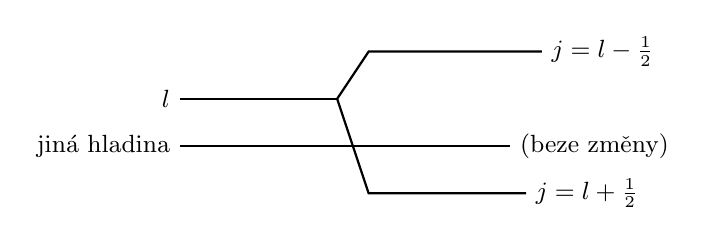
\begin{tikzpicture}[scale=1]
  \draw[thick] (0,1) -- (2,1);
  \draw[thick] (0,0.4) -- (4.2,0.4);
  \draw[thick] (2,1) -- (2.4,1.6) -- (4.6,1.6);
  \draw[thick] (2,1) -- (2.4,-0.2) -- (4.4,-0.2);
  \node[left] at (0,1) {\small \(l\)};
  \node[left] at (0,0.4) {\small jiná hladina};
  \node[right] at (4.6,1.6) {\small \(j=l-\frac12\)};
  \node[right] at (4.4,-0.2) {\small \(j=l+\frac12\)};
  \node[right] at (4.2,0.4) {\small (beze změny)};
\end{tikzpicture}
\end{center}

Takto upravené pořadí hladin vede ke správným uzavřeným slupkám:
\begin{veta}[Magická čísla]
\[
  \vzorec{\text{magická čísla: } 2,\ 8,\ 20,\ 28,\ 50,\ 82,\ 126}
\]
Příklady (dvojnásobně magických) jader: \({}^{4}_{2}\mathrm{He}\),
\({}^{208}_{82}\mathrm{Pb}\) (\(Z=82\), \(N=126\)).
\end{veta}
Např.\ číslo 28 vzniká tak, že hladina \(1f_{7/2}\) (\(l=3\), 8 nukleonů)
se odštěpí od zbytku slupky \(n=3\) a uzavře se samostatně: \(20+8=28\).

\paragraph{Spin a parita jader ze slupkového modelu.} Slupkový model umí
předpovědět \(J^P\) základního stavu:
\begin{itemize}
  \item S-S: \(J^P = 0^+\) (všechny nukleony spárované);
  \item L-S, S-L: spárované nukleony nepřispívají, \(J^P\) jádra je dán
    \emph{posledním nepárovým nukleonem}: \(J=j\) a \(P=(-1)^l\).
\end{itemize}

\strana{P03-7}
\begin{priklad}[\({}^{15}_{8}\mathrm{O}\)]
\({}^{15}_{8}\mathrm{O}\): 8 protonů \(\to\) nepřispěje (zaplněné
slupky \(1s_{1/2}\), \(1p_{3/2}\), \(1p_{1/2}\)). 7 neutronů ano, ale jak?
Neutrony zaplňují hladiny odspodu:
\begin{center}
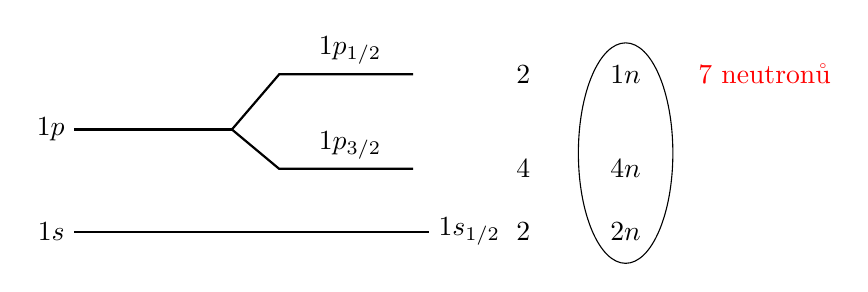
\begin{tikzpicture}[scale=1]
  \draw[thick] (0,0) -- (4.5,0);
  \node[left] at (0,0) {\(1s\)};
  \node[right] at (4.5,0) {\(1s_{1/2}\)};
  \draw[thick] (0,1.3) -- (2,1.3);
  \node[left] at (0,1.3) {\(1p\)};
  \draw[thick] (2,1.3) -- (2.6,2) -- (4.3,2);
  \draw[thick] (2,1.3) -- (2.6,0.8) -- (4.3,0.8);
  \node[above] at (3.5,2) {\(1p_{1/2}\)};
  \node[above] at (3.5,0.8) {\(1p_{3/2}\)};
  \node at (5.7,2) {2};
  \node at (5.7,0.8) {4};
  \node at (5.7,0) {2};
  \node at (7,2) {\(1n\)};
  \node at (7,0.8) {\(4n\)};
  \node at (7,0) {\(2n\)};
  \draw (7,1) ellipse (0.6 and 1.4);
  \node[red,right] at (7.8,2) {7 neutronů};
\end{tikzpicture}
\end{center}
(prostřední sloupec: kapacita \(2j+1\) hladiny; vpravo obsazení neutrony).
Hladiny \(1s_{1/2}\) a \(1p_{3/2}\) jsou plné (spárované), poslední neutron
sedí sám v \(1p_{1/2}\): \(j=\tfrac12\), \(l=1\Rightarrow P=-1\). Tedy
\[
  \color{red} J^P\big({}^{15}_{8}\mathrm{O}\big) = \tfrac12^- ,
\]
v souladu s experimentem. (Ekvivalentně: \({}^{15}\)O je
\uv{\({}^{16}\)O minus jeden neutron} -- díra v \(1p_{1/2}\).)
\end{priklad}

\subsection{Kolektivní stavy}

Excitované stavy jádra nemusí vznikat jen přeskokem jednoho nukleonu na
vyšší hladinu. Jádro jako celek (mnoho nukleonů současně, \uv{kolektivně})
může:
\begin{itemize}
  \item \kw{vibrovat} -- povrch kmitá kolem rovnovážného (kulového) tvaru;
  \item \kw{rotovat} -- pokud je jádro deformované (nekulové), může rotovat
    kolem osy kolmé k ose symetrie.
\end{itemize}

\begin{center}
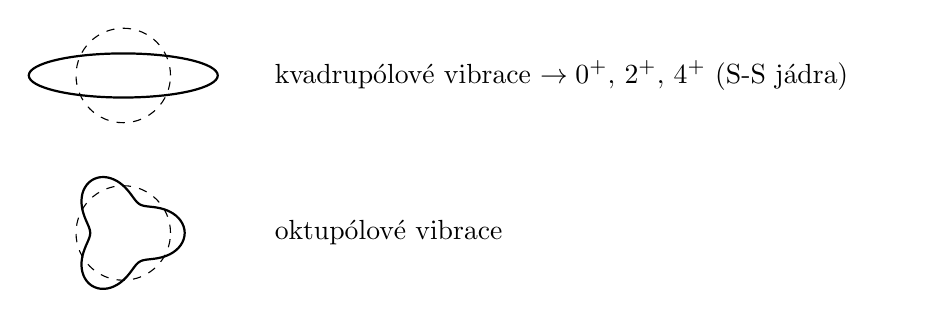
\begin{tikzpicture}
  % kvadrupol
  \draw[thick] (0,0) ellipse (1.2 and 0.28);
  \draw[dashed] (0,0) circle (0.6);
  \node[right,text width=8cm] at (1.8,0) {\kw{kvadrupólové vibrace} \(\to 0^+,\,2^+,\,4^+\) (S-S jádra)};
  % oktupol
  \begin{scope}[yshift=-2cm]
    \draw[thick,domain=0:360,samples=120,smooth] plot ({\x}:{0.6*(1+0.3*cos(3*\x))});
    \draw[dashed] (0,0) circle (0.6);
    \node[right] at (1.8,0) {\kw{oktupólové vibrace}};
  \end{scope}
\end{tikzpicture}
\end{center}

Při \kw{kvadrupólových vibracích} (multipolarita \(\lambda=2\)) kmitá kulové
jádro mezi zploštělým a protáhlým elipsoidem. Kvantum vibrace (\uv{fonon})
nese moment hybnosti 2 a kladnou paritu; stav s jedním fononem je tedy
\(2^+\), dvoufononové stavy tvoří triplet \(0^+,2^+,4^+\). Energie hladin jsou
přibližně ekvidistantní (harmonický oscilátor). U S-S jader je mezi
základním stavem \(0^+\) a prvními jednočásticovými excitacemi mezera
(rozbití páru stojí energii), proto jsou vibrační pásy dobře
identifikovatelné. \kw{Oktupólové vibrace} (\(\lambda=3\), tvar
\uv{hrušky}) mají fonon \(3^-\) a jsou vzácnější.

\begin{vysvetleni}[Rotační pásy]
Deformované jádro s momentem setrvačnosti \(\mathcal I\) rotuje s energií
\(E_{\text{rot}} = \frac{\hbar^2}{2\mathcal I}J(J+1)\). Kolem osy symetrie
rotovat nemůže (kvantově nelze rozlišit natočení symetrického objektu), proto
jen kolem osy kolmé. U S-S deformovaných jader jsou nejnižší hladiny
rotační, opět \(0^+,2^+,4^+,\dots\), ale -- na rozdíl od vibrací -- nejsou
ekvidistantní: rozdíly rostou jako \(J(J+1)\), tj.\ poměr
\(E(4^+)/E(2^+)=20/6\approx3{,}33\) (vibrace: \(\approx2\)). Podle tohoto
poměru se v experimentu rozliší vibrační a rotační jádra (viz Davídkovy
slajdy \uv{Vibrační a rotační pásy}).
\end{vysvetleni}
